\documentclass[11pt]{article}

\usepackage[top=1in, bottom=1in, left=1in, right=1in]{geometry}
\usepackage{amsfonts}
\usepackage{graphicx}
\usepackage{float}
\usepackage[utf8]{inputenc}
\usepackage[section]{placeins}
\usepackage{abstract}
\usepackage{amsmath}
\usepackage{amsfonts}
\usepackage{amssymb}
\usepackage{enumitem}
\renewcommand{\abstractnamefont}{\normalfont\bfseries} 
\renewcommand{\abstracttextfont}{\normalfont} 
\numberwithin{equation}{section}
\newcommand{\argmax}{\operatornamewithlimits{argmax}}

\begin{document}

\title{DMUU Project Report}
\author{\begin{tabular}{cc}
Roland Hellström & Sebastian Ånerud \\
XXXXXX-xxxx & 910407-5958 \\
asdf.comasd@ & anerud@student.chalmers.se
\end{tabular}}
\date{\today}
\maketitle

\begin{flushleft}

\section{Introduction}

This project consists of building an agent that is able to act and take optimal decisions in unknown and arbitrary environments. The only thing known about the environments, that the agent is supposed to act in, is the number of states, the number of actions and that the underlying model is a Markov Decision Process. Also it is known that one of the environments is a Partially Observable MDP (POMDP). However, the agent presented in this report does not implement any algorithm specifically designed to act well in such an environment.

\section{Method}

very much methods. so amaze. wow.

\section{Results}

very much results. so amaze. wow. \newline 

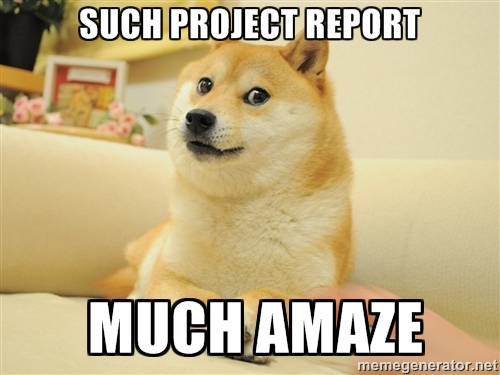
\includegraphics[scale=1]{DOGE}

\section{Discussion}

very much discuss. so amaze. wow.

\section{Conclusion}

very much conclude. so amaze. wow.

\end{flushleft}

\end{document}